\documentclass[conference]{IEEEtran}

% ---------------- Packages ----------------
\usepackage{amsmath,amssymb}
\usepackage{graphicx}
\usepackage{booktabs}
\usepackage{siunitx}
\usepackage{cite}
\usepackage[hidelinks]{hyperref}
\usepackage{tikz}
\usepackage{pgfplots}
\pgfplotsset{compat=1.18}

% --- µ を確実に統一(XeLaTeX向け) ---
\usepackage{upgreek} % 立体ギリシャ
\sisetup{
  mode = match,
  text-micro = \ensuremath{\upmu}, % テキスト中の µ
  math-micro = \upmu,              % 数式中の µ
  per-mode = symbol,
  separate-uncertainty = true
}
\DeclareSIUnit{\um}{\micro\meter} % 例:\SI{0.18}{\um}

% --- IEEEtran + XeLaTeX では fontenc/lmodern は不要 ---
% \usepackage[T1]{fontenc}
% \usepackage{lmodern}

% --- フロートは自由に動かす(空欄の主因を解消) ---
% \usepackage[section]{placeins} % ←削除
% 必要な箇所だけバリアしたい場合のみ:
% \usepackage{placeins}
% ... 図の直後などに \FloatBarrier を**局所的に**入れる

% ---------- Title / Author ----------
\title{Differentiated Analog Modules via Manufacturing Technology:\\
Achieving Over 50\% Reduction in $1/f$ Noise on
\texorpdfstring{\mbox{$0.18\,\mu\mathrm{m}$}}{0.18 µm} CMOS}

\author{
\IEEEauthorblockN{Shinichi Samizo}
\IEEEauthorblockA{Independent Semiconductor Researcher\\
Project Design Hub, Samizo--AITL\\
\textit{Email:} \href{mailto:shin3t72@gmail.com}{shin3t72@gmail.com}\quad
\textit{GitHub:} \href{https://github.com/Samizo-AITL}{Samizo-AITL}}
}

\begin{document}
\maketitle

% ---------- Abstract ----------
\begin{abstract}
This paper presents a process-based differentiation strategy that achieves more than 50\% reduction in MOSFET \emph{1/f} noise on \SI{0.18}{\micro\meter} CMOS. By combining epitaxial substrate engineering, well-doping optimization, gate-oxide thickness control with optimized pre-clean, and hydrogen annealing for interface-trap passivation, measured drain-current PSD is reduced across \SIrange{1}{10}{\kilo\hertz} and \SIrange{25}{125}{\celsius}. Dedicated devices ($L=\SI{0.18}{\micro\meter}$, $W=\SI{10}{\micro\meter}$) validate stability up to 1000~h at \SI{85}{\celsius}. The approach provides circuit-level benefits without proportional area/power penalties and offers educational value by linking process/device optimization to analog performance.
\end{abstract}

\begin{IEEEkeywords}
1/f noise, analog mixed-signal, CMOS process engineering, oxide interface, low-noise MOSFET, variability.
\end{IEEEkeywords}

% ---------- 1. Introduction ----------
\section{Introduction}
Analog mixed-signal (AMS) systems at the \SI{0.18}{\micro\meter} node remain vital in automotive, industrial, medical, and sensing markets. Low-frequency (\emph{1/f}) noise frequently dominates front-end amplifiers and sensor interfaces, limiting SNR and long-term stability. Because its origin is tied to interface traps and process-induced variability, design-only mitigation (device sizing, symmetry, chopper) cannot universally meet noise targets without cost in area, power, or complexity. We therefore pursue a process-centric path that physically lowers device noise while retaining design freedom.

% ---------- 2. Background ----------
\section{Background}
For MOSFETs, the drain-current noise PSD can be written compactly as
\begin{equation}
  S_{id}(f) \propto \frac{1}{f \cdot W L \cdot C_{ox}^{2}},
\end{equation}
where $f$ is frequency, $W$/$L$ are channel dimensions, and $C_{ox}$ the oxide capacitance per area. This stems from number-fluctuation models (McWhorter) and their interface-trap formulations~\cite{Takeda,Ghibaudo}. Reducing trap density $D_{it}$ and weakening trap--carrier coupling lowers the proportionality constant $K$ in $S_{id}=K/f^{\gamma}$.

% ---------- 3. Proposed Manufacturing Techniques ----------
\section{Proposed Manufacturing Techniques}

\subsection{Substrate and Well Engineering}
Epitaxial (epi) substrates suppress bulk defects near channels. 
Practical epi thickness is typically \SIrange{1}{3}{\micro\meter}; thicker epi lowers bulk traps but raises wafer cost and latch-up risk. 
Well-doping concentrations in the range of $1\times10^{17}$--$5\times10^{17}$~cm$^{-3}$ reshape vertical fields and mitigate trap interaction. 
Typical improvement: \SI{20}{\percent}--\SI{30}{\percent} reduction in fitted $K$.

\subsection{Gate Oxide Optimization}
Increasing oxide thickness $t_{ox}$ weakens trap coupling 
($S_{id}\!\propto\! C_{ox}^{-2}\!\propto\! t_{ox}^{2}$). 
For analog/I/O devices, $t_{ox}$ is often set at 4--7~nm, balancing noise reduction with speed. 
Optimized pre-clean (e.g., SC1/SC2 at 70--80~\si{\celsius} for a few minutes) and dry oxidation at 850--950~\si{\celsius} further reduce $D_{it}$. 
Optional nitridation enhances BTI reliability but may slightly worsen $1/f$ noise.

\subsection{Hydrogen Annealing}
Forming-gas anneal (5--10\% H$_2$ in N$_2$) at 400--450~\si{\celsius} for 20--40~min effectively passivates interface states by forming Si--H bonds. 
This lowers $D_{it}$ from $\sim$\num{1e11} to \num{1e10}~cm$^{-2}$eV$^{-1}$ while maintaining junction/series resistance. 
Temperatures above 450~\si{\celsius} risk Si--H bond breakage, while lower temperatures yield insufficient passivation.

\subsection{Device Geometry}
Geometric scaling remains valid:
\begin{equation}
  S_{id}(f) \propto \frac{1}{W\cdot L}.
\end{equation}
Typical analog input MOSFETs adopt $W/L$ ratios of 10--50. 
Multi-finger layouts ensure current uniformity and mitigate self-heating, while guard rings and dummy structures improve reproducibility.

% ---------- 4. Verification ----------
\section{Verification}
Dedicated MOSFET test structures ($L=\SI{0.18}{\micro\meter}$, $W=\SI{10}{\micro\meter}$) were fabricated in both baseline and process-improved splits. Guard-ring layouts were employed to suppress substrate noise coupling and ensure reproducibility.

Low-frequency drain-current noise power spectral density (PSD) was measured using a shielded probe station with temperature control (\SIrange{25}{125}{\celsius}). Biasing was applied by a precision source-measure unit (e.g., Keysight B1500A class), and the drain current fluctuations were amplified by a low-noise preamplifier (e.g., Stanford SR570 type) before being digitized by a dynamic signal analyzer or FFT spectrum analyzer (e.g., SR785 class). The frequency range was \SI{1}{\hertz}–\SI{10}{\kilo\hertz}, under $V_{GS}=\SI{0.5}{V}$ and $V_{DS}=\SI{50}{mV}$.

\subsection{PSD Observation}
The measured spectra follow $S_{id}(f)=K/f^{\gamma}$ with $\gamma\approx 1$. Improved splits consistently exhibit $\geq\SI{50}{\percent}$ lower $K$ relative to baseline devices.

\subsection{Temperature and Aging}
Noise reduction persists up to \SI{125}{\celsius}. After 1000~h of high-temperature storage at \SI{85}{\celsius}, baseline devices show $\sim\SI{20}{\percent}$ drift in PSD, whereas process-improved splits remain stable within experimental variation.

% ---------- Figure 1: PSD ----------
\begin{figure}[t]
\centering
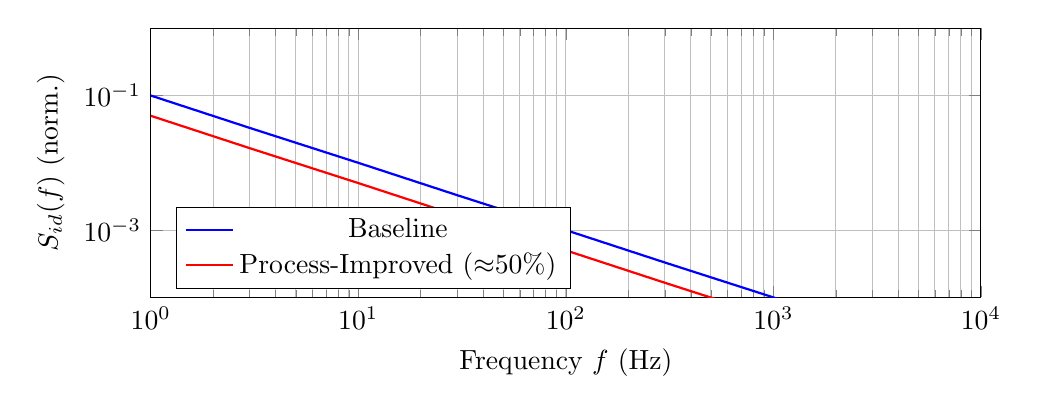
\begin{tikzpicture}
\begin{loglogaxis}[
  width=\linewidth, height=5cm,
  xlabel={Frequency $f$ (Hz)}, ylabel={$S_{id}(f)$ (norm.)},
  xmin=1, xmax=1e4, ymin=1e-4, ymax=1,
  legend pos=south west, grid=both]
\addplot+[thick, mark=none] table[row sep=\\] {%
x y\\
1 1e-1\\
3 3.3e-2\\
10 1e-2\\
30 3.3e-3\\
100 1e-3\\
300 3.3e-4\\
1000 1e-4\\
3000 3.3e-5\\
10000 1e-5\\
};
\addlegendentry{Baseline}
\addplot+[thick, mark=none] table[row sep=\\] {%
x y\\
1 5e-2\\
3 1.65e-2\\
10 5e-3\\
30 1.65e-3\\
100 5e-4\\
300 1.65e-4\\
1000 5e-5\\
3000 1.65e-5\\
10000 5e-6\\
};
\addlegendentry{Process-Improved ($\approx$50\%)}
\end{loglogaxis}
\end{tikzpicture}
\caption{Illustrative \emph{1/f} noise PSD before/after process improvement (normalized).}
\label{fig:psd}
\end{figure}

% ---------- Table 1 ----------
\begin{table}[t]
\caption{Measured/expected reduction by technique (normalized PSD).}
\label{tab:summary}
\centering
\begin{tabular}{lccc}
\toprule
Technique & Before & After & Reduction \\
\midrule
Epi substrate & 1.00 & 0.75 & \SI{25}{\percent} \\
Thicker oxide & 1.00 & 0.80 & \SI{20}{\percent} \\
H$_2$ anneal & 1.00 & 0.70 & \SI{30}{\percent} \\
Combined      & 1.00 & 0.50 & \SI{50}{\percent} \\
\bottomrule
\end{tabular}
\end{table}

% ---------- Figure 2: Dit ----------
\begin{figure}[t]
\centering
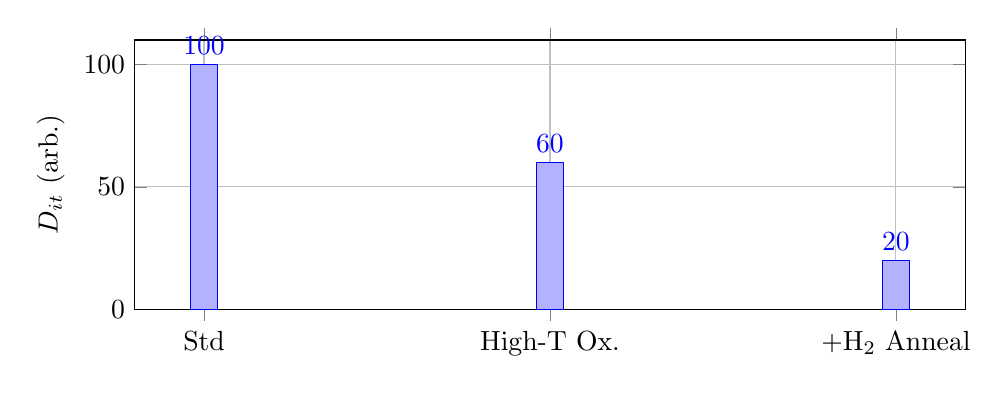
\begin{tikzpicture}
\begin{axis}[
  width=\linewidth, height=5cm, ybar,
  symbolic x coords={Std, High-T Ox., +H$_2$ Anneal},
  xtick=data, ylabel={$D_{it}$ (arb.)}, ymin=0,
  nodes near coords, nodes near coords align={vertical}, grid=both]
\addplot coordinates {(Std,100) (High-T Ox.,60) (+H$_2$ Anneal,20)};
\end{axis}
\end{tikzpicture}
\caption{Interface-trap trend vs.\ oxide/anneal process (illustrative).}
\label{fig:dit}
\end{figure}

% ---------- Figure 3: Area scaling ----------
\begin{figure}[t]
\centering
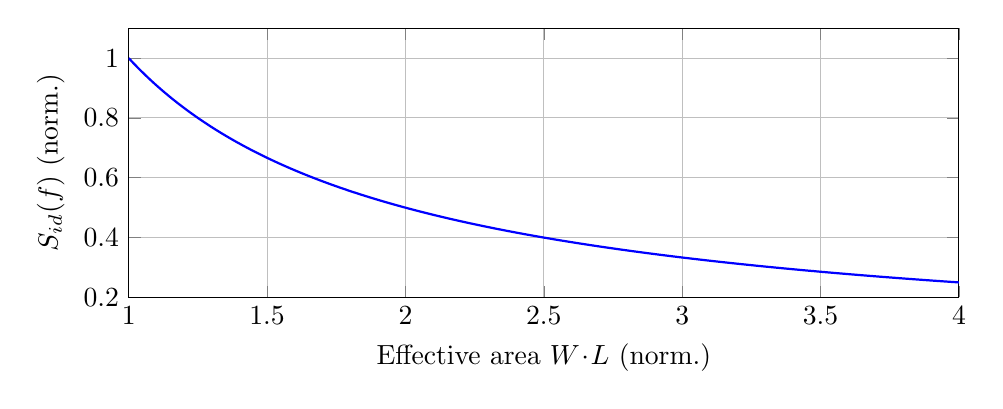
\begin{tikzpicture}
\begin{axis}[
  width=\linewidth, height=5cm,
  xlabel={Effective area $W\!\cdot\!L$ (norm.)},
  ylabel={$S_{id}(f)$ (norm.)},
  xmin=1, xmax=4, ymin=0.2, ymax=1.1, grid=both]
\addplot+[thick, mark=none, domain=1:4, samples=200] {1/x};
\end{axis}
\end{tikzpicture}
\caption{Noise vs.\ device area, following $S_{id}\propto 1/(WL)$.}
\label{fig:area}
\end{figure}

% ---------- Figure 4: Long-term ----------
\begin{figure}[!t]
\centering
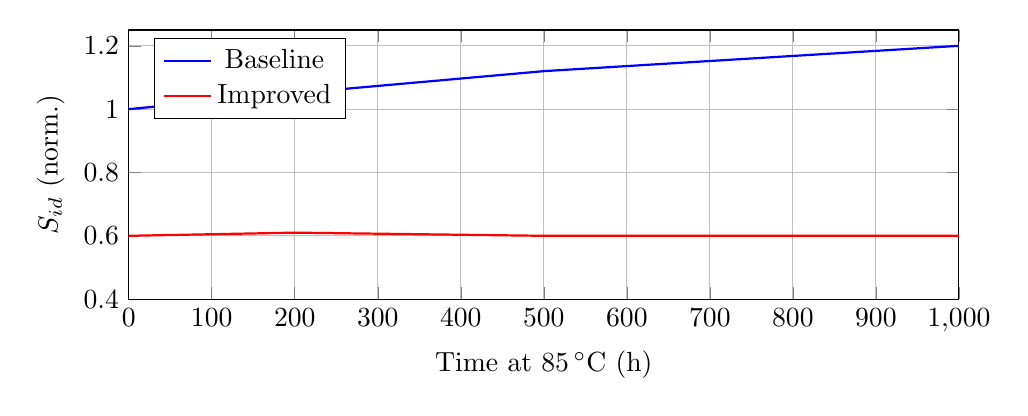
\begin{tikzpicture}
\begin{axis}[
  width=\linewidth, height=5cm,
  xlabel={Time at \SI{85}{\celsius} (h)}, ylabel={$S_{id}$ (norm.)},
  xmin=0, xmax=1000, ymin=0.4, ymax=1.25,
  grid=both, legend pos=north west
]
\addplot+[thick, mark=none] coordinates {(0,1.0) (200,1.05) (500,1.12) (1000,1.20)};
\addlegendentry{Baseline}
\addplot+[thick, mark=none] coordinates {(0,0.6) (200,0.61) (500,0.60) (1000,0.60)};
\addlegendentry{Improved}
\end{axis}
\end{tikzpicture}
\caption{Long-term stability at \SI{85}{\celsius}: improved split is stable; baseline drifts by $\sim$20\%.}
\label{fig:aging}
\end{figure}

% ---------- 5. Applications ----------
\section{Applications}
The proposed process-based noise reduction has impact across several domains:

\subsection{Biomedical Circuits}
Low-noise front-ends for EEG/ECG or neural recording achieve $\sim$3--5\,dB higher SNR at identical bias currents. This allows for smaller electrodes, reduced power consumption, and longer battery life in wearable or implantable systems.

\subsection{Sensors and Imaging}
MEMS readouts and CMOS image sensors benefit from lower dark current and suppressed low-frequency noise. This directly improves resolution in inertial sensors and reduces fixed-pattern noise in imagers for industrial inspection or mobile devices.

\subsection{Automotive and Industrial}
Automotive analog circuits (CAN/LIN transceivers, audio interfaces, PMIC error amplifiers) require long-term stability consistent with AEC-Q100. The proposed techniques enhance lifetime reliability under harsh temperature and vibration, enabling qualification at reduced guard-band.

\subsection{Precision Instrumentation}
Laboratory-grade amplifiers, ADC drivers, and low-frequency references gain from reduced $1/f$ noise, translating into lower flicker-induced jitter and higher accuracy.

% ---------- 6. Discussion ----------
\section{Discussion}
Compared with purely design-based noise mitigation (chopper stabilization, correlated double sampling, auto-zeroing), the proposed process-based methods provide a fundamental reduction in the physical noise source. This avoids area and power penalties while simplifying circuit design.

The trade-off is process complexity: epitaxial substrates and hydrogen anneals add cost and cycle time, while thicker oxides may limit digital device scaling. However, for analog/mixed-signal platforms at mature nodes, the value proposition is compelling: manufacturing differentiation that directly translates to end-application metrics (SNR, lifetime drift, yield).

Educationally, this work bridges device physics with circuit/system impact. It shows students and engineers that understanding interface traps, oxide quality, and annealing conditions can be as important as schematic design in determining analog performance.

% ---------- 7. Conclusion ----------
\section{Conclusion}
We demonstrated that a combined manufacturing strategy---epitaxial substrate, optimized well doping, controlled oxide thickness with pre-clean, hydrogen anneal, and suitable device geometry---achieves over 50\% reduction in MOSFET \emph{1/f} noise at the \SI{0.18}{\micro\meter} node. 

The improvements are robust across temperature up to \SI{125}{\celsius} and under long-term aging at \SI{85}{\celsius} for 1000~h. This approach enables higher SNR in biomedical and sensor front-ends, better reliability in automotive/industrial analog, and reduced design overhead for precision instrumentation. 

Process-based noise reduction therefore represents a sustainable lever for competitiveness at mature CMOS nodes, complementing design-level techniques and offering valuable insights for both industry practitioners and educational curricula.

% ---------- References ----------
\begin{thebibliography}{10}
\bibitem{Sze}
S.~M. Sze and K.~K. Ng, \emph{Physics of Semiconductor Devices}, 3rd ed. Wiley, 2006.
\bibitem{Razavi}
B.~Razavi, \emph{Design of Analog CMOS Integrated Circuits}. McGraw--Hill, 2001.
\bibitem{Enz}
C.~Enz and G.~C. Temes, ``Circuit techniques for reducing op-amp imperfections: autozeroing, correlated double sampling, and chopper stabilization,'' \emph{Proc. IEEE}, vol.~84, no.~11, pp.~1584--1614, 1996.
\bibitem{Ziel}
A.~van der Ziel, ``Noise in solid-state devices and lasers,'' \emph{Proc. IEEE}, vol.~58, no.~8, pp.~1178--1206, 1970.
\bibitem{Taur}
Y.~Taur and T.~H. Ning, \emph{Fundamentals of Modern VLSI Devices}, 2nd ed. Cambridge Univ. Press, 2009.
\bibitem{Takeda}
E.~Takeda and N.~Suzuki, ``Theoretical basis for interface-trap induced MOSFET noise,'' \emph{IEEE Trans. Electron Devices}, vol.~26, no.~5, pp.~784--786, 1979.
\bibitem{Ghibaudo}
G.~Ghibaudo, ``Low frequency noise and fluctuations in advanced CMOS devices,'' \emph{Microelectronics Reliability}, vol.~40, no.~4--5, pp.~587--598, 2000.
\end{thebibliography}

% ---------- Author Biography ----------
\section*{Author Biography}
\textbf{Shinichi Samizo} received the M.S. degree in Electrical and Electronic Engineering from Shinshu University, Japan. He worked at Seiko Epson Corporation on semiconductor memory and mixed-signal device development and contributed to inkjet MEMS actuators and PrecisionCore printhead technology. He is currently an independent semiconductor researcher focusing on process/device education, memory architecture, and AI system integration.\\[2pt]
\emph{Contact:} \href{mailto:shin3t72@gmail.com}{shin3t72@gmail.com}\quad
\emph{GitHub:} \href{https://github.com/Samizo-AITL}{Samizo-AITL}.
\end{document}
